\ifpdf
    \graphicspath{{Chapter7/Figs/Raster/}{Chapter7/Figs/PDF/}{Chapter7/Figs/}}
\else
    \graphicspath{{Chapter7/Figs/Vector/}{Chapter7/Figs/}}
\fi

\chapter{Preliminary Online Experiment}
\label{ch7}
\section{Introduction}
\label{ch7:sec:intr}

As delineated in the preceding chapter, a preliminary experimental phase was conducted to empirically determine the preferred interaction distances for German and Italian cohorts relative to a Baseline group. 
This study was facilitated via the Prolific~\footnote{\href{https://www.prolific.com/}{https://www.prolific.com/}} crowdsourcing platform. 
The methodological framework described herein serves as a foundational precursor to the primary investigation regarding socially-aware navigation and environmental interaction.

This chapter provides a comprehensive description of the experimental protocol, the structured questionnaires employed, and the specific inclusion and exclusion criteria for participant selection. 
Subsequently, the empirical results are presented, followed by a critical analysis and discussion of the findings.

\section{Experiments}
\label{ch7:sec:exps}

The primary objective of this investigation is to establish a ground truth regarding the preferred interaction distances for two specific national cultures: German and Italian. 
By quantifying these proxemic preferences under controlled conditions, we aim to validate the empirical basis for the cultural parameters integrated into the robot's navigation and adaptation modules.

The study commences with a questionnaire incorporating the same metrics detailed in Section~\ref{ch5:sec:measuring_cultural_competence}. 
Following the initial assessment, participants are presented with six video recordings—rendered as high-quality GIFs—captured from a static camera perspective. 
These videos depict the Pepper robot navigating between two points within a room and executing a return trajectory.
The navigational algorithm employed in these stimuli is identical to the RRT*-based system described in Section~\ref{ch6:sec:navigation} and utilized in the subsequent main study. 
Participants were tasked with rating each interaction on a 5-point Likert scale. 
To assess proxemic preferences, the videos were varied according to the robot’s minimum distance from the human, ranging from $0.42\text{m}$ to $1.5\text{m}$ in equidistant increments.

To maintain experimental rigor, each stimulus was recorded featuring both male and female subjects. 
For each participant, one of the two subjects was randomly assigned to mitigate potential gender-related biases or interaction effects. 
These recordings were formally classified as third-person perspective data, as they allowed participants to evaluate the interaction from an external, objective viewpoint.

Furthermore, the assessment incorporated static imagery captured from an egocentric perspective to approximate a first-person view (FPV). 
This simulated the visual experience of a user interacting directly with the robot at the same discrete comfort intervals utilized in the video stimuli. 
These images were formally categorized as first-person perspective data.

\section{Results}\label{ch7:sec:res}The preliminary online study involved a total of 36 participants, comprising 17 Italian and 19 German nationals. 
Table~\ref{ch7:tab:online_study_res} presents the descriptive statistics, including the mean and standard deviation, disaggregated by question and cultural cohort. To evaluate the statistical significance and magnitude of the observed differences, we performed a Kolmogorov-Smirnov (KS) Test and calculated Cliff’s Delta, reporting the resulting $p$-values, $d$-values, and the corresponding effect size for each metric.

\begin{table}[]
\centering
\begin{tabular}{l S[table-format=1.2] S[table-format=1.2] S[table-format=1.2] S[table-format=1.2] S[table-format=1.2] c r}
\toprule
& \multicolumn{2}{c}{Mean} & \multicolumn{2}{c}{Std. Dev.} & {KS Test} & \multicolumn{2}{c}{Cliff's Delta} \\
\cmidrule(lr){2-3} \cmidrule(lr){4-5} \cmidrule(lr){7-8}
Question & {IT} & {DE} & {IT} & {DE} & {$p$-value} & {$d$} & {Effect} \\
\midrule
Country & 0.51 & 0.52 & 0.23 & 0.19 & 0.99 & -0.06 & Negligible \\
Language & 0.79 & 0.73 & 0.22 & 0.22 & 0.88 & 0.20 & Small \\
Culture & 0.65 & 0.54 & 0.21 & 0.21 & 0.63 & 0.26 & Small \\
\addlinespace
Video 1 & 0.37 & 0.35 & 0.16 & 0.16 & 1.00 & 0.09 & Negligible \\
\addlinespace
Video 2 & 0.27 & 0.30 & 0.14 & 0.16 & 0.95 & -0.17 & Small \\
\addlinespace
Video 3 & 0.38 & 0.40 & 0.14 & 0.15 & 0.88 & -0.11 & Negligible \\
\addlinespace
Video 4 & 0.51 & 0.53 & 0.14 & 0.15 & 0.88 & -0.07 & Negligible \\
\addlinespace
Video 5 & 0.54 & 0.51 & 0.13 & 0.15 & 0.75 & 0.11 & Negligible \\
\addlinespace
Video 6 & 0.50 & 0.44 & 0.20 & 0.20 & 0.88 & 0.18 & Small \\
\addlinespace
Image 1 & 0.24 & 0.24 & 0.19 & 0.18 & 1.00 & -0.01 & Negligible \\
\addlinespace
Image 2 & 0.37 & 0.40 & 0.18 & 0.18 & 0.97 & -0.09 & Negligible \\
\addlinespace
Image 3 & 0.44 & 0.40 & 0.13 & 0.14 & 0.91 & 0.16 & Small \\
\addlinespace
Image 4 & 0.42 & 0.46 & 0.12 & 0.17 & 0.75 & -0.15 & Small \\
\addlinespace
Image 5 & 0.40 & 0.39 & 0.20 & 0.19 & 1.00 & 0.03 & Negligible \\
\addlinespace
Image 6 & 0.36 & 0.32 & 0.23 & 0.21 & 0.73 & 0.07 & Negligible \\
\bottomrule
\end{tabular}
\caption{Statistics of the results of the online study for each question and each national culture.}
\label{ch7:tab:online_study_res}
\end{table}

Figure~\ref{ch7:fig:culture_answeres_distributions} illustrates the probability distributions regarding the degree to which German and Italian participants identify with their respective national territories, languages, and cultures, alongside the aggregate sample average.

\begin{figure*}
\centering
\begin{subfigure}[b]{0.75\columnwidth}
\centering
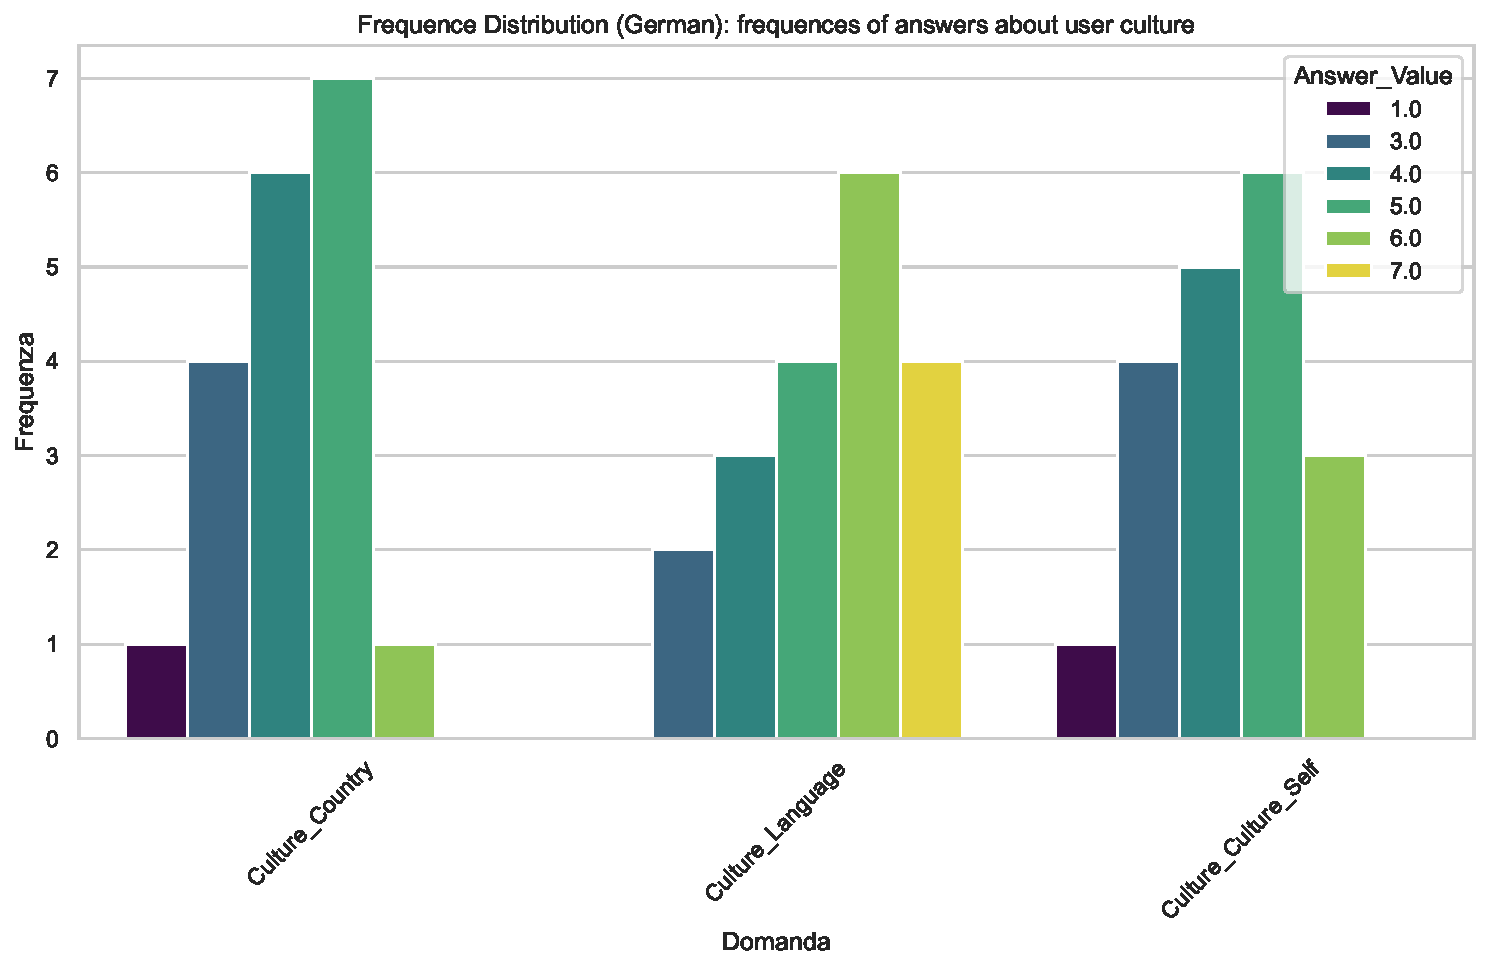
\includegraphics[width=\columnwidth]{Chapter7/Figs/frequences of answers about user culture_German.pdf}
\caption{Germans answers distribution on subjects assessment of culture.}
\end{subfigure} \\
\begin{subfigure}[b]{0.75\columnwidth}
\centering
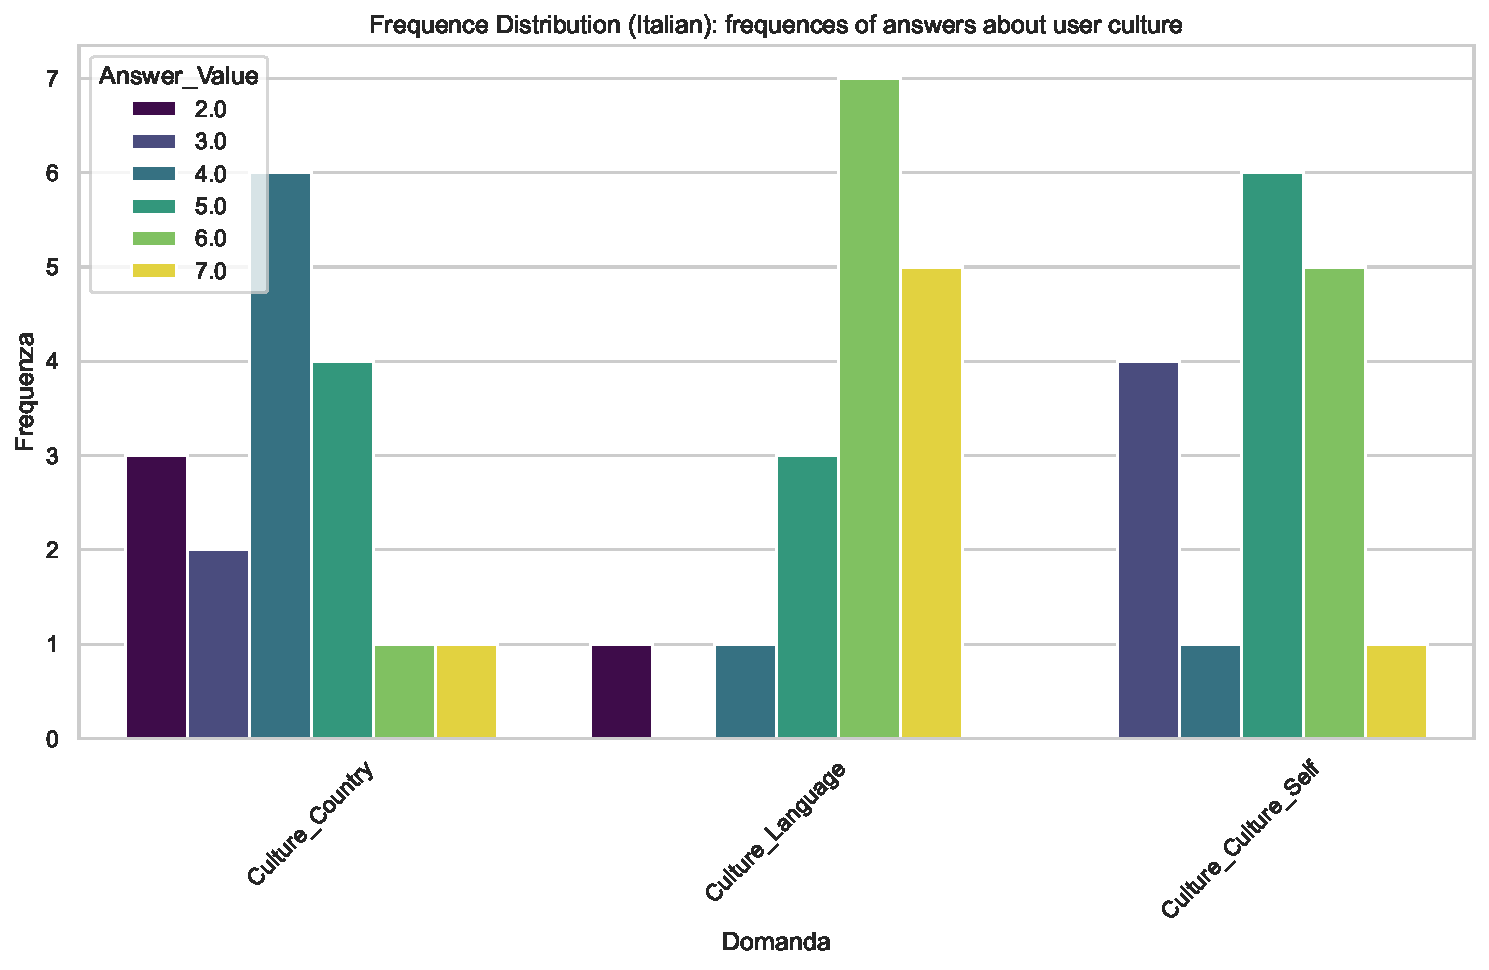
\includegraphics[width=\columnwidth]{Chapter7/Figs/frequences of answers about user culture_Italian.pdf}
\caption{Italian answers distribution on subjects assessment of culture.}
\end{subfigure} \\
\begin{subfigure}[b]{0.75\columnwidth}
\centering
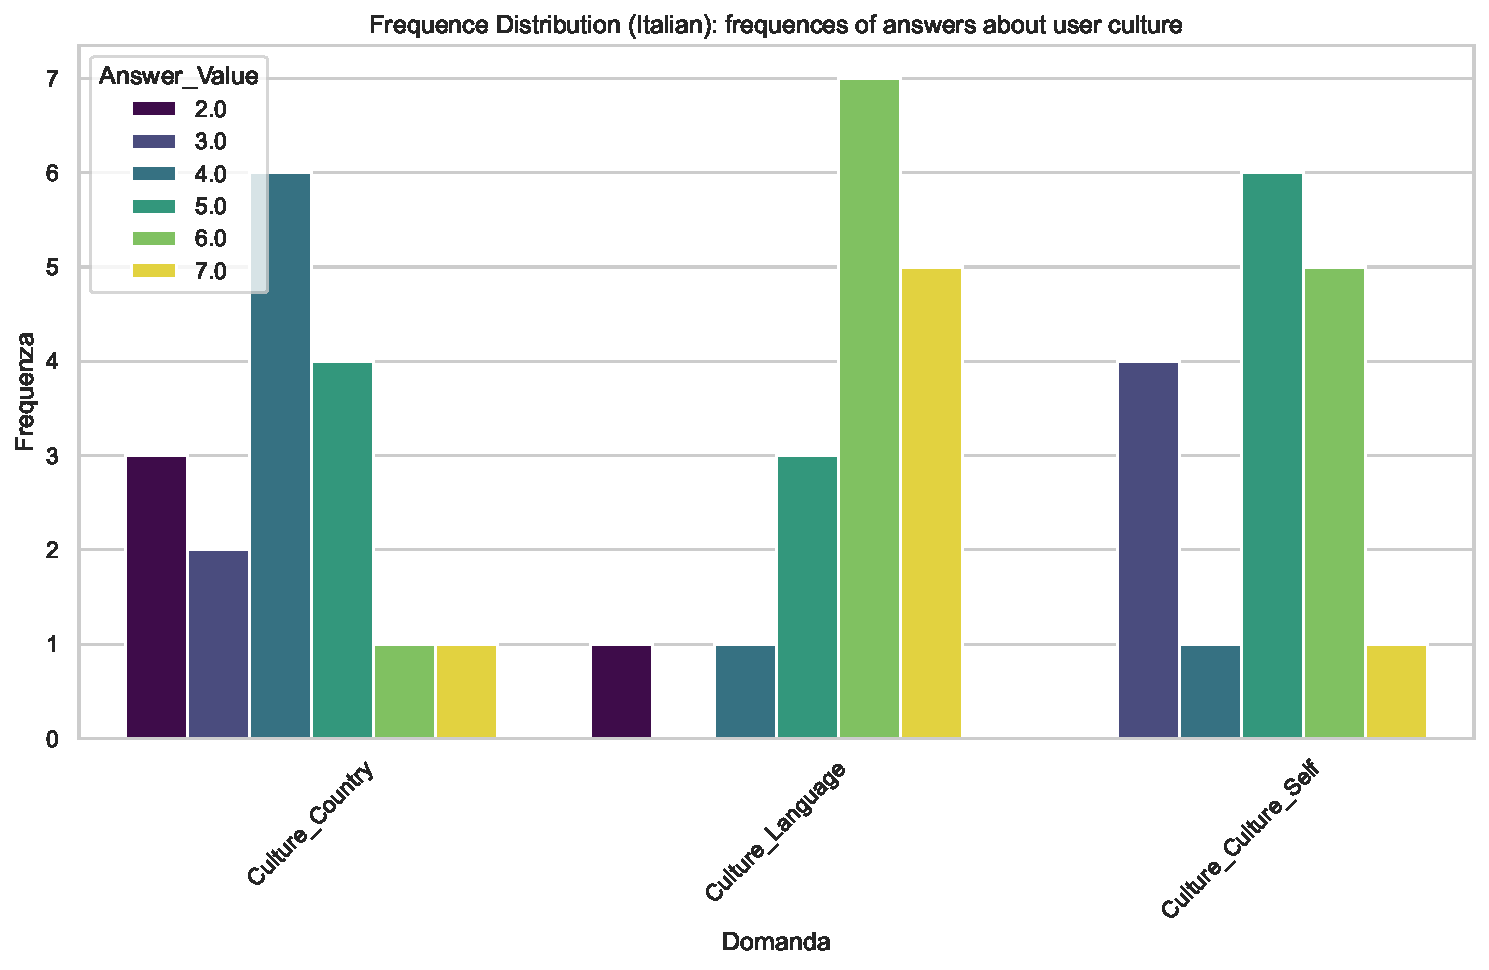
\includegraphics[width=\columnwidth]{Chapter7/Figs/frequences of answers about user culture_Italian.pdf}
\caption{Global answers distribution on subjects assessment of culture.}
\end{subfigure}
\caption{Distributions of the answers on the questions related to on subjects culture.}
\label{ch7:fig:culture_answeres_distributions}
\end{figure*}

Figure~\ref{ch7:fig:1st_view_answeres_distributions} illustrates the probability distributions of preferences for both German and Italian cohorts, as well as the aggregate sample average, regarding the robot's proximity distances. 
These data points were captured while participants evaluated static imagery from an egocentric (first-person) perspective.

\begin{figure*}
\centering
\begin{subfigure}[b]{0.75\columnwidth}
\centering
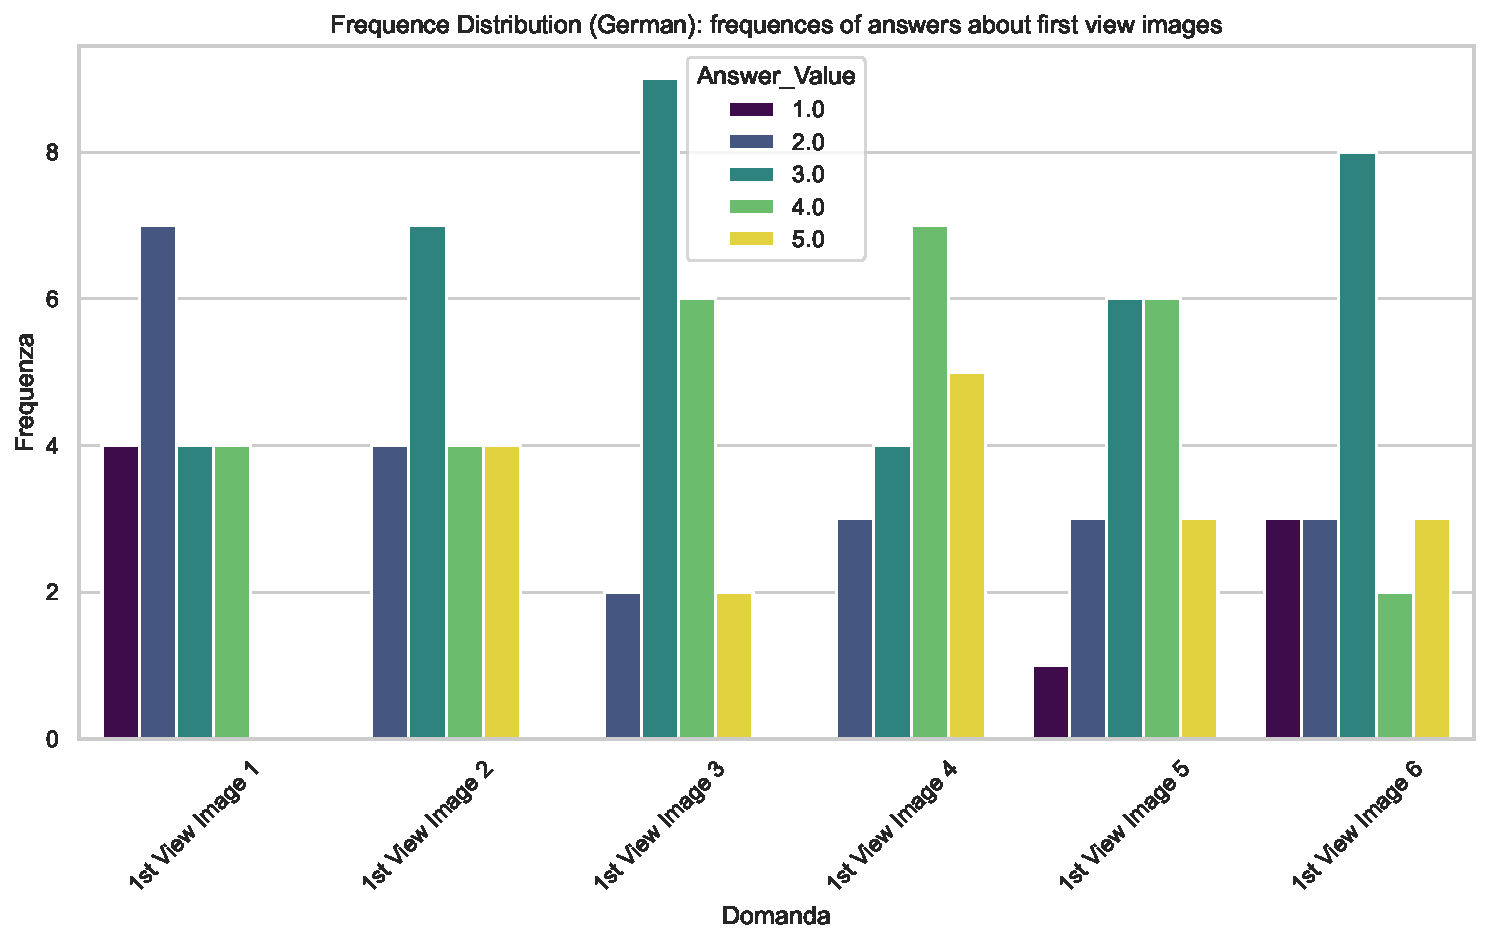
\includegraphics[width=\columnwidth]{Chapter7/Figs/frequences of answers about first view images_German.pdf}
\caption{Germans answers distribution on $1^{st}$ View Images.}
\end{subfigure} \\
\begin{subfigure}[b]{0.75\columnwidth}
\centering
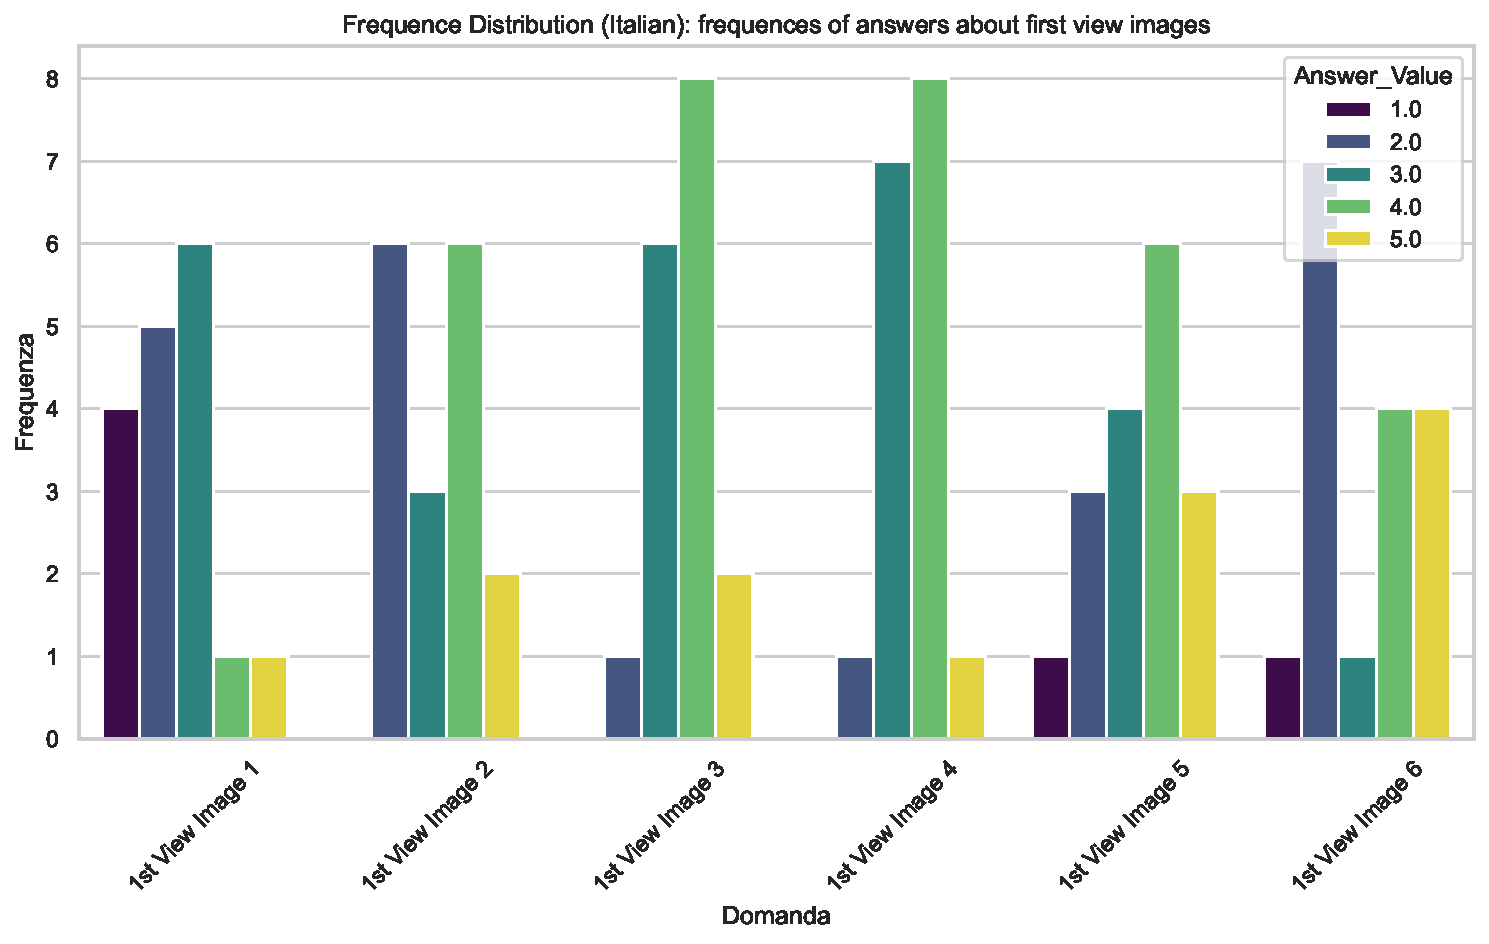
\includegraphics[width=\columnwidth]{Chapter7/Figs/frequences of answers about first view images_Italian.pdf}
\caption{Italian answers distribution on $1^{st}$ View Images.}
\end{subfigure} \\
\begin{subfigure}[b]{0.75\columnwidth}
\centering
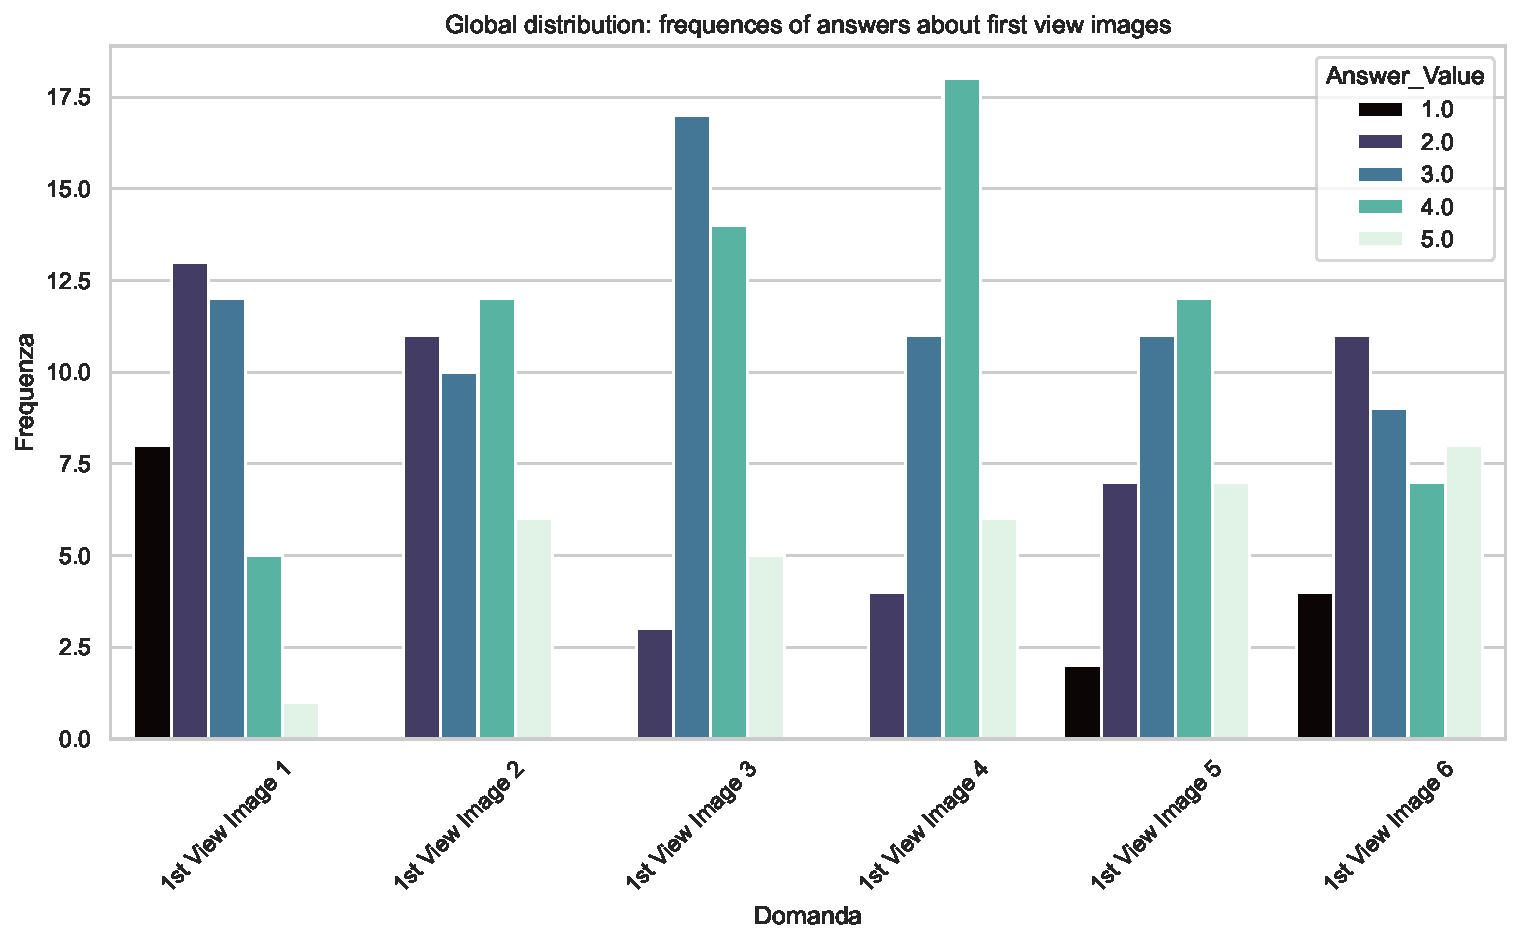
\includegraphics[width=\columnwidth]{Chapter7/Figs/frequences of answers about first view images_GLOBALE.pdf}
\caption{Global answers distribution on $1^{st}$ View Images.}
\end{subfigure}
\caption{Distributions of the answers on the questions related to $1^{st}$ View Images.}
\label{ch7:fig:1st_view_answeres_distributions}
\end{figure*}

Figure~\ref{ch7:fig:3rd_view_answeres_distributions} illustrates the probability distributions of preferences for German and Italian cohorts, as well as the aggregate sample average, regarding the robot's proximity distances. 
These ratings were elicited while participants observed video sequences of the robot navigating a bidirectional trajectory between two points from a third-person perspective. 

\begin{figure*}
\centering
\begin{subfigure}[b]{0.75\columnwidth}
\centering
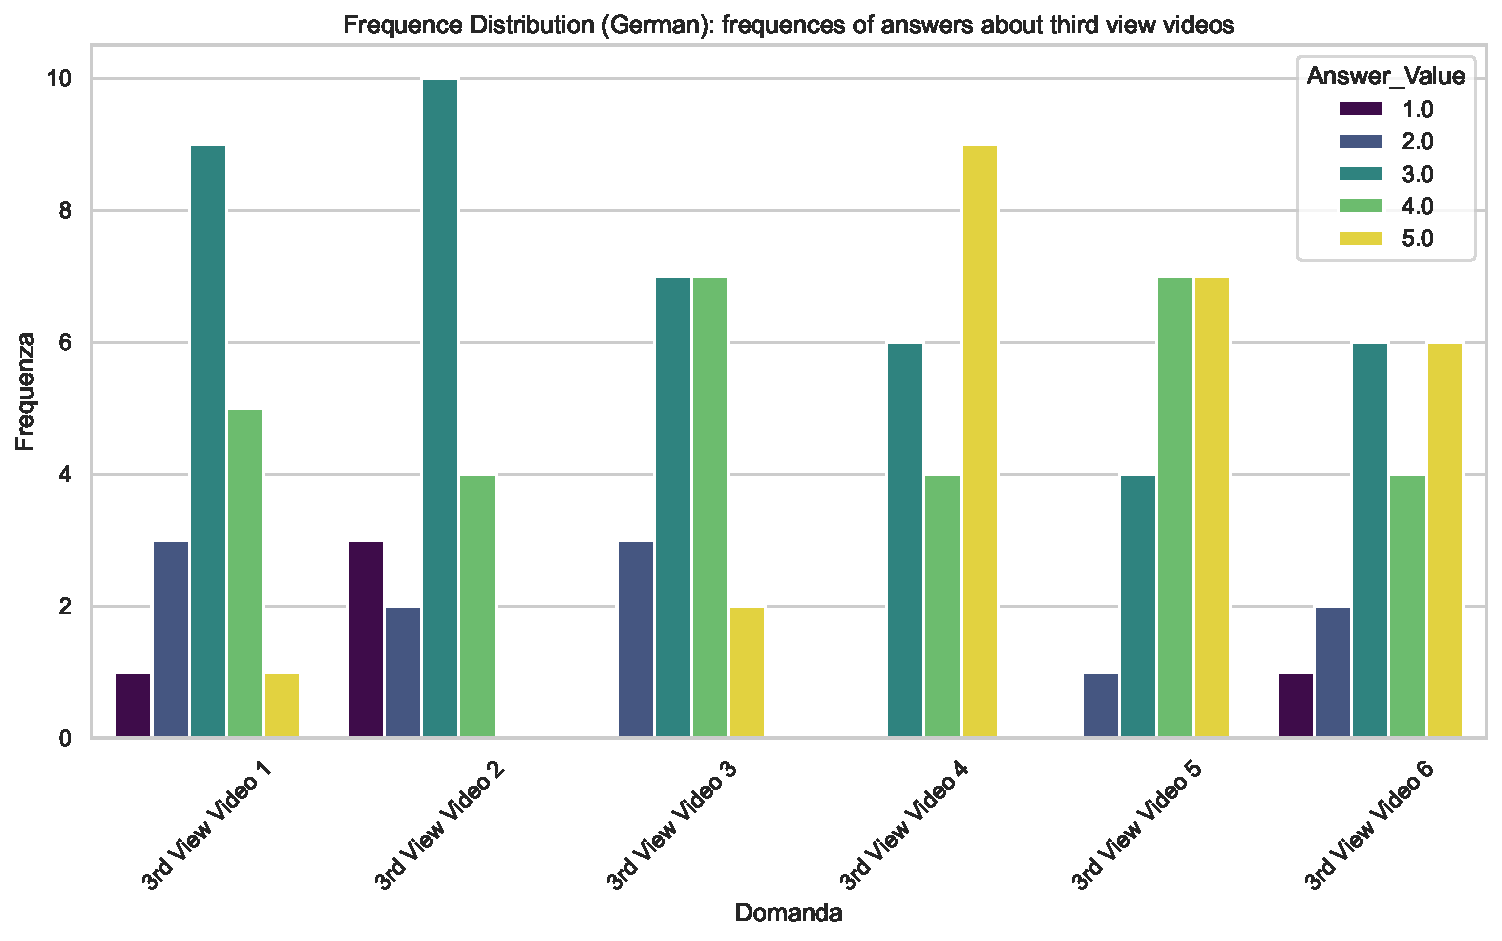
\includegraphics[width=\columnwidth]{Chapter7/Figs/frequences of answers about third view videos_German.pdf}
\caption{Germans answers distribution on $3^{rd}$ View Videos.}
\end{subfigure} \\
\begin{subfigure}[b]{0.75\columnwidth}
\centering
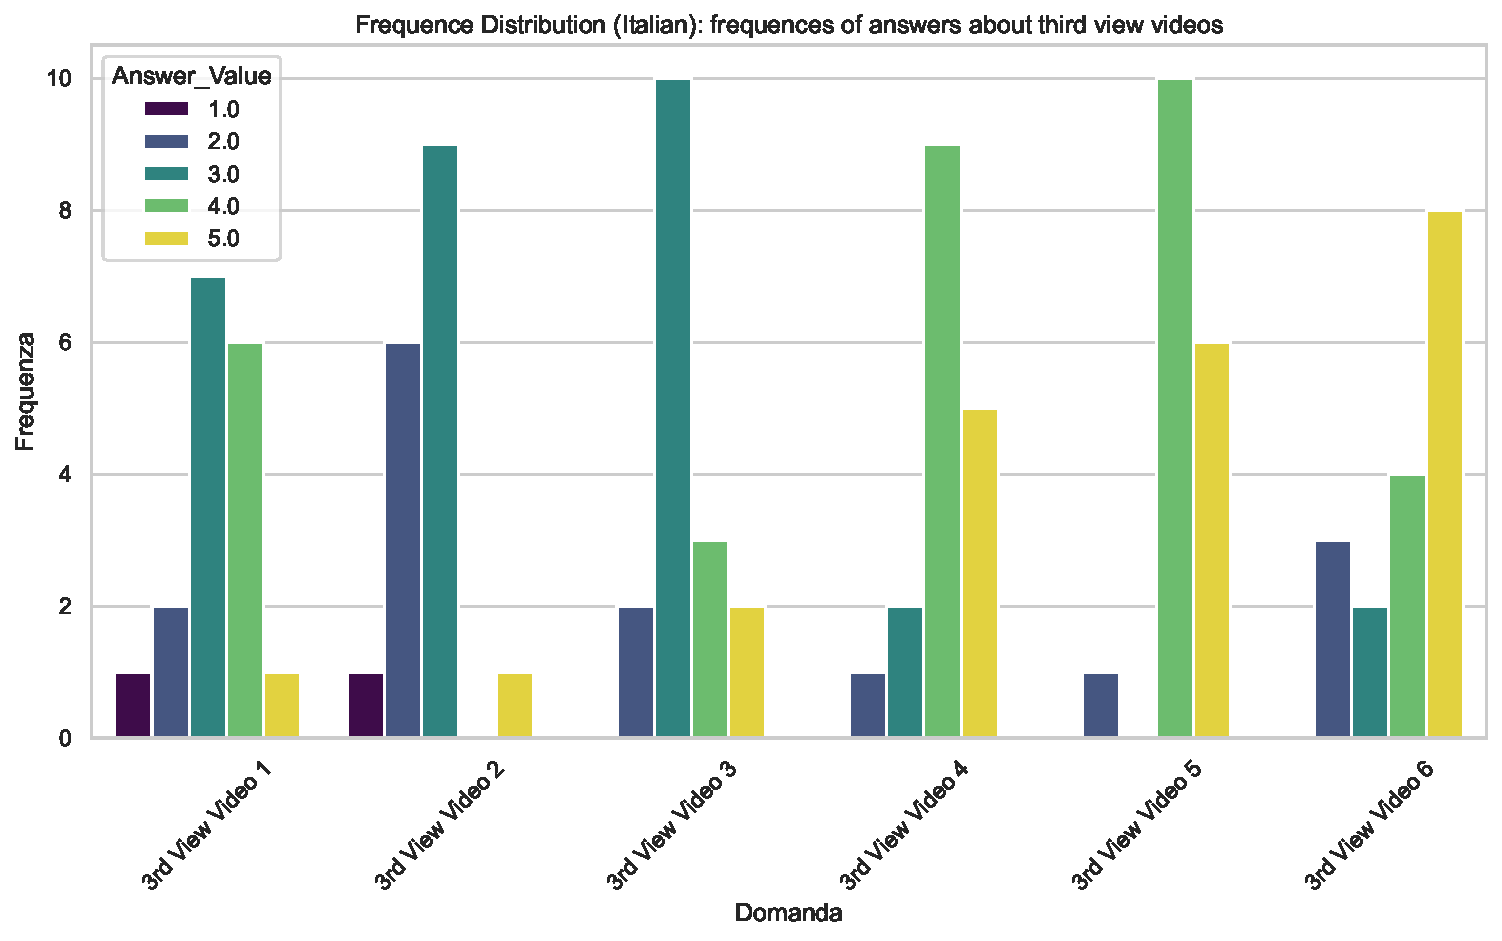
\includegraphics[width=\columnwidth]{Chapter7/Figs/frequences of answers about third view videos_Italian.pdf}
\caption{Italian answers distribution on  $3^{rd}$ View Videos.}
\end{subfigure} \\
\begin{subfigure}[b]{0.75\columnwidth}
\centering
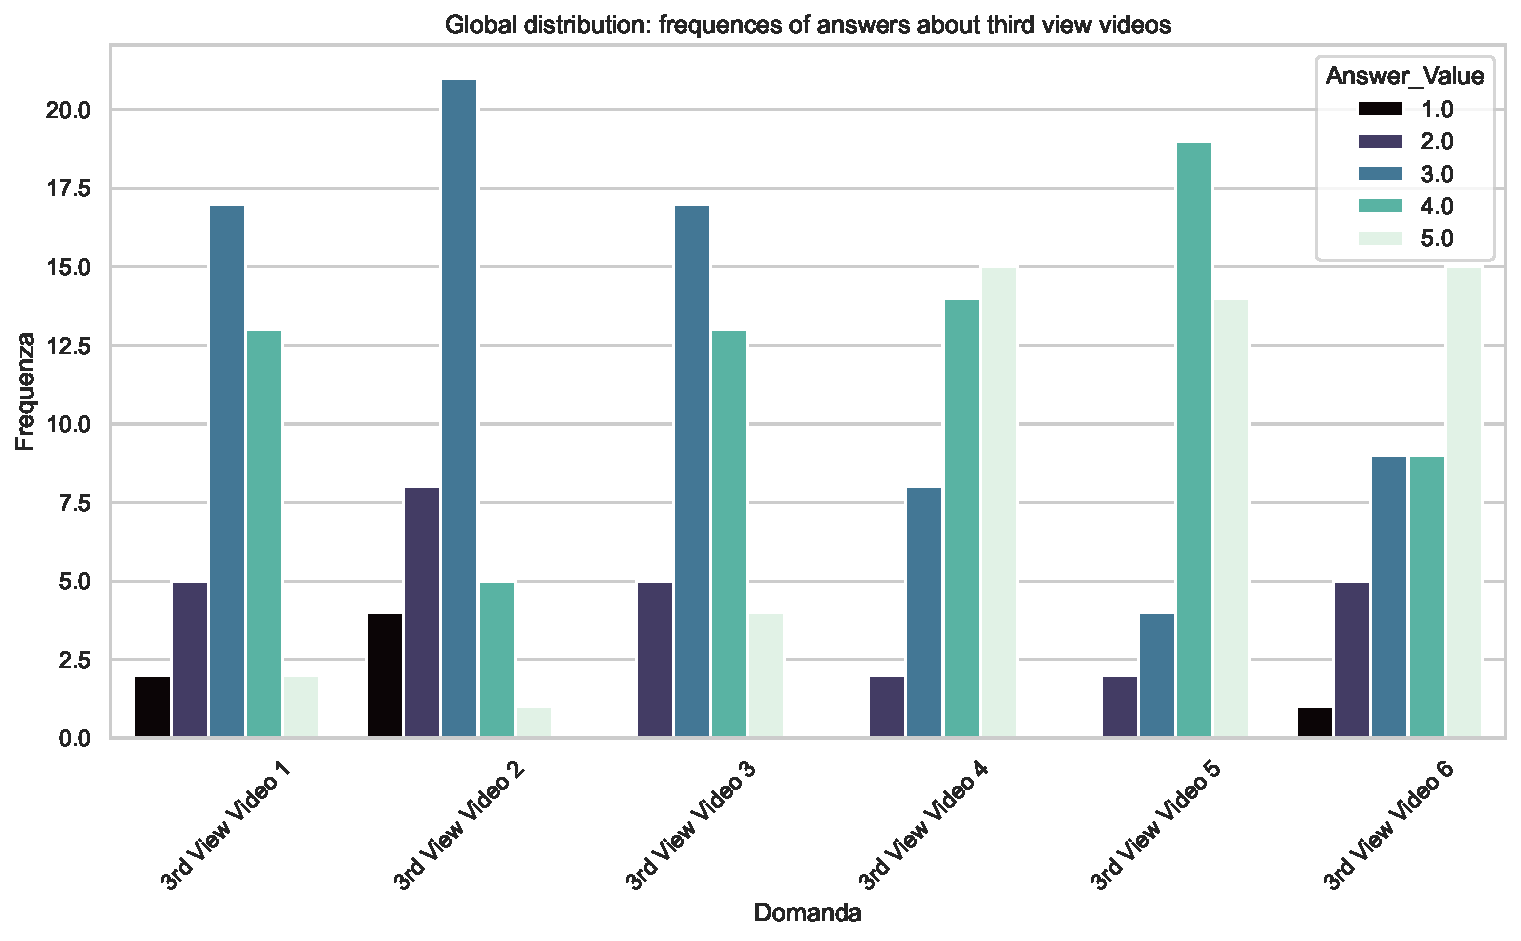
\includegraphics[width=\columnwidth]{Chapter7/Figs/frequences of answers about third view videos_GLOBALE.pdf}
\caption{Global answers distribution on  $3^{rd}$ View Videos.}
\end{subfigure}
\caption{Distributions of the answers on the questions related to  $3^{rd}$ View Videos.}
\label{ch7:fig:3rd_view_answeres_distributions}
\end{figure*}

The empirical findings derived from this preliminary study demonstrate significant intrinsic value. 
An analysis of the data distributions reveals distinct variances between the German and Italian cohorts regarding their proxemic and communicative preferences. 
These disparities are corroborated by the statistical results presented in Table~\ref{ch7:tab:online_study_res}, which identifies specific metrics where the distribution shift reaches statistical significance between the two cultures. 
Furthermore, the results indicate that these cross-cultural differences are mitigated as the cohorts converge toward a unified consensus on certain neutral parameters.

\begin{comment}
    %
\begin{table}[ht]
\centering
{\footnotesize
\begin{tabular}{lll}
\toprule
q$_i$ & Italian & German \\
\midrule
q1 & \makecell[l]{Quale immagine descrive meglio il tuo rapporto\\ con [paese]?} & \makecell[l]{Welches Bild beschreibt Ihre Beziehung\\ zu [Land] am besten?} \\
q2 & \makecell[l]{Quale immagine descrive meglio il tuo rapporto\\ con [lingua]?} & \makecell[l]{Welches Bild beschreibt Ihre Beziehung\\ zu [Sprache] am besten?} \\ 
q3 & \makecell[l]{Quale immagine descrive meglio il tuo rapporto\\ con [cultura]?} & \makecell[l]{Welches Bild beschreibt Ihre Beziehung\\ zu [Kultur] am besten?} \\
q4 & \makecell[l]{Valuta quanto bene il robot mantiene una distanza\\ appropriata dall'umano  (1 è il peggiore, 5 è il migliore).} & \makecell[l]{Bewerten Sie, wie gut der Roboter einen\\ angemessenen Abstand zum Menschen\\ einhält (1 ist der Hammer, 5 ist der Beste).} \\
q5 & \makecell[l]{Valuta quanto bene il robot mantiene una distanza\\ appropriata dall'umano  (1 è il peggiore, 5 è il migliore).} & \makecell[l]{Bewerten Sie, wie gut der Roboter einen\\ angemessenen Abstand zum Menschen\\ einhält (1 ist der Hammer, 5 ist der Beste).} \\
q6 & \makecell[l]{Valuta quanto bene il robot mantiene una distanza\\ appropriata dall'umano  (1 è il peggiore, 5 è il migliore).} & \makecell[l]{Bewerten Sie, wie gut der Roboter einen\\ angemessenen Abstand zum Menschen\\ einhält (1 ist der Hammer, 5 ist der Beste).} \\
q7 & \makecell[l]{Valuta quanto bene il robot mantiene una distanza\\ appropriata dall'umano  (1 è il peggiore, 5 è il migliore).} & \makecell[l]{Bewerten Sie, wie gut der Roboter einen\\ angemessenen Abstand zum Menschen\\ einhält (1 ist der Hammer, 5 ist der Beste).} \\
q8 & \makecell[l]{Valuta quanto bene il robot mantiene una distanza\\ appropriata dall'umano  (1 è il peggiore, 5 è il migliore).} & \makecell[l]{Bewerten Sie, wie gut der Roboter einen\\ angemessenen Abstand zum Menschen\\ einhält (1 ist der Hammer, 5 ist der Beste).} \\
q10 & \makecell[l]{Valuta quanto bene il robot mantiene una distanza\\ appropriata da te  (1 è il peggiore, 5 è il migliore). Così è\\ come vedresti il robot dalla tua prospettiva.} & \makecell[l]{Bewerten Sie, wie gut der Roboter einen\\ angemessenen Abstand zu Ihnen einhält\\ (1 ist der Hammer, 5 ist der Beste). Das ist\\ so, dass der Roboter Ihr Ziel verlässt.} \\
q10 & \makecell[l]{Valuta quanto bene il robot mantiene una distanza\\ appropriata da te  (1 è il peggiore, 5 è il migliore). Così è\\ come vedresti il robot dalla tua prospettiva.} & \makecell[l]{Bewerten Sie, wie gut der Roboter einen\\ angemessenen Abstand zu Ihnen einhält\\ (1 ist der Hammer, 5 ist der Beste). Das ist\\ so, dass der Roboter Ihr Ziel verlässt.} \\
q11 & \makecell[l]{Valuta quanto bene il robot mantiene una distanza\\ appropriata da te  (1 è il peggiore, 5 è il migliore). Così è\\ come vedresti il robot dalla tua prospettiva.} & \makecell[l]{Bewerten Sie, wie gut der Roboter einen\\ angemessenen Abstand zu Ihnen einhält\\ (1 ist der Hammer, 5 ist der Beste). Das ist\\ so, dass der Roboter Ihr Ziel verlässt} \\
q12 & \makecell[l]{Valuta quanto bene il robot mantiene una distanza\\ appropriata da te  (1 è il peggiore, 5 è il migliore). Così è\\ come vedresti il robot dalla tua prospettiva.} & \makecell[l]{Bewerten Sie, wie gut der Roboter einen\\ angemessenen Abstand zu Ihnen einhält\\ (1 ist der Hammer, 5 ist der Beste). Das ist\\ so, dass der Roboter Ihr Ziel verlässt} \\
q13 & \makecell[l]{Valuta quanto bene il robot mantiene una distanza\\ appropriata da te  (1 è il peggiore, 5 è il migliore). Così è\\ come vedresti il robot dalla tua prospettiva.} & \makecell[l]{Bewerten Sie, wie gut der Roboter einen\\ angemessenen Abstand zu Ihnen einhält\\ (1 ist der Hammer, 5 ist der Beste). Das ist\\ so, dass der Roboter Ihr Ziel verlässt} \\
q14 & \makecell[l]{Valuta quanto bene il robot mantiene una distanza\\ appropriata da te  (1 è il peggiore, 5 è il migliore). Così è\\ come vedresti il robot dalla tua prospettiva.} & \makecell[l]{Bewerten Sie, wie gut der Roboter einen\\ angemessenen Abstand zu Ihnen einhält\\ (1 ist der Hammer, 5 ist der Beste). Das ist\\ so, dass der Roboter Ihr Ziel verlässt} \\
q15 & \makecell[l]{Valuta quanto bene il robot mantiene una distanza\\ appropriata da te  (1 è il peggiore, 5 è il migliore). Così è\\ come vedresti il robot dalla tua prospettiva.} & \makecell[l]{Bewerten Sie, wie gut der Roboter einen\\ angemessenen Abstand zu Ihnen einhält\\ (1 ist der Hammer, 5 ist der Beste). Das ist\\ so, dass der Roboter Ihr Ziel verlässt} \\
\bottomrule
\end{tabular}
}
\caption{Question index (use q1, q2 ... in other tables)}
\label{tab:questions_index}
\end{table}
%
\end{comment}

\begin{comment}
    \begin{landscape}
\begin{table}[ht]
\centering
{\scriptsize
\begin{tabular}{rrrrrrrrrrrrrrlrrl}
\toprule
q$_i$ &  $\mu_i$ & $\mu_g$ & $\sigma_i$ & $\sigma_g$ & $\Delta_\mu$ & shapiro$_{a_p}$ & shapiro$_{b_p}$ & levene$_p$ & mannwhitney$_u$ & mannwhitney$_p$ & ass. & chosen\_test & chosen\_stat & chosen\_p  \\
\midrule
q1 &  4.300 & 4.273 & 1.636 & 0.905    & 0.027 & 0.627 & 0.001 & 0.167 & 55.500 & 1.000 & F & mannwhitney & 55.500 & 1.000  \\
q2 & 5.400 & 5.273 & 1.578 & 1.272    & 0.127 & 0.141 & 0.518 & 0.601 & 60.500 & 0.718 & T & t-test & 0.204 & 0.840  \\
q3 &  4.700 & 4.636 & 1.567 & 0.924    & 0.064 & 0.037 & 0.217 & 0.091 & 57.000 & 0.913 & F & mannwhitney & 57.000 & 0.913  \\
q4 &  3.300 & 3.364 & 1.160 & 1.120    & -0.064 & 0.328 & 0.141 & 0.830 & 53.000 & 0.911 & T & t-test & -0.128 & 0.900  \\
q5 &  2.800 & 2.818 & 1.033 & 1.079    & -0.018 & 0.043 & 0.032 & 0.724 & 50.000 & 0.731 & F & mannwhitney & 50.000 & 0.731 \\
q6 & 3.100 & 3.636 & 0.876 & 0.924    & -0.536 & 0.026 & 0.217 & 0.451 & 36.000 & 0.164 & F & mannwhitney & 36.000 & 0.164 \\
q7 &  3.700 & 4.091 & 0.823 & 0.944    & -0.391 & 0.045 & 0.002 & 0.215 & 42.500 & 0.373 & F & mannwhitney & 42.500 & 0.373 \\
q8 & 4.200 & 3.909 & 0.919 & 1.044    & 0.291 & 0.004 & 0.079 & 0.452 & 64.000 & 0.525 & F & mannwhitney & 64.000 & 0.525 \\
q9 & 4.000 & 3.545 & 1.247 & 1.368    & 0.455 & 0.008 & 0.084 & 0.820 & 65.000 & 0.482 & F & mannwhitney & 65.000 & 0.482 \\
q10 & 2.600 & 2.818 & 1.265 & 1.079    & -0.218 & 0.445 & 0.047 & 0.743 & 48.000 & 0.636 & F & mannwhitney & 48.000 & 0.636 \\
q11 & 3.200 & 3.818 & 1.135 & 0.874    & -0.618 & 0.029 & 0.006 & 0.224 & 38.000 & 0.228 & F & mannwhitney & 38.000 & 0.228 \\
q12 & 3.600 & 3.818 & 0.699 & 0.751    & -0.218 & 0.008 & 0.018 & 0.778 & 46.000 & 0.514 & F & mannwhitney & 46.000 & 0.514 \\
q13 & 3.600 & 3.727 & 0.843 & 1.104    & -0.127 & 0.172 & 0.097 & 0.500 & 49.500 & 0.711 & T & t-test & -0.295 & 0.772 \\
q14 & 3.500 & 3.091 & 1.354 & 0.944    & 0.409 & 0.276 & 0.095 & 0.138 & 67.500 & 0.380 & T & t-test & 0.810 & 0.428 \\
q15 &3.100 & 2.636 & 1.524 & 0.924    & 0.464 & 0.055 & 0.004 & 0.061 & 61.000 & 0.687 & F & mannwhitney & 61.000 & 0.687 \\
\bottomrule
\end{tabular}}
\caption{Full corresponding question diagnostics and test results}
\label{tab:corresponding_full}
\end{table}
\end{landscape}
%
%
\begin{table}[ht]
\centering
\begin{tabular}{llllrr}
\toprule
group & italiano & deutsch & test & stat & p \\
\midrule
culture & {'n': 10, 'mean': 4.8, 'std': 1.5169820591889789, 'median': 5.0} & {'n': 11, 'mean': 4.7272727272727275, 'std': 0.8668997355606654, 'median': 4.666666666666667} & t-test & 0.137 & 0.893 \\
\bottomrule
\end{tabular}
\caption{Culture group summary and test}
\label{tab:culture}
\end{table}

\begin{table}[ht]
\centering
\begin{tabular}{lllrrlrrrl}
\toprule
group & italiano\_cols & deutsch\_cols & n\_italiano & n\_deutsch & test & stat & p & cohen\_d & diagnostics \\
\midrule
culture & ['q1', '', 'q3'] & ['Welches Bild beschreibt Ihre Beziehung zu [Land] am besten?', 'q2', 'q3'] & 10 & 11 & t-test & 0.137 & 0.893 & 0.060 & {'shapiro\_a\_p': 0.8766233016250535, 'shapiro\_b\_p': 0.6334003315165518, 'levene\_p': 0.12117239597133107, 'mannwhitney\_u': 58.0, 'mannwhitney\_p': 0.8598076138526077, 'assumptions\_ok': True} \\
videos & [] & [] & 0 & 0 &  &  &  &  &  \\
images & [] & [] & 0 & 0 &  &  &  &  &  \\
\bottomrule
\end{tabular}
\caption{Automatic group comparisons}
\label{tab:groups_auto}
\end{table}

\begin{table}[ht]
\centering
\begin{tabular}{lrrlrrr}
\toprule
group & n\_italiano & n\_deutsch & test & stat & p & cohen\_d \\
\midrule
culture & 10 & 11 & t-test & 0.137 & 0.893 & 0.060 \\
videos & 0 & 0 &  &  &  &  \\
images & 0 & 0 &  &  &  &  \\
\bottomrule
\end{tabular}
\caption{Group comparisons (means and tests)}
\label{tab:groups}
\end{table}

\begin{table}[ht]
\centering
\begin{tabular}{llrrrr}
\toprule
comparison & test\_used & u & p & n\_a & n\_b \\
\midrule
Deutsch vs Italiano & mannwhitney & 12678.000 & 0.700 & 165 & 150 \\
\bottomrule
\end{tabular}
\caption{Per-language comparison results (flat)}
\label{tab:perlang}
\end{table}
\begin{table}[ht]
\centering
\begin{tabular}{lrrlrrr}
\toprule
q\_label & question\_index & mean\_diff & chosen\_test & chosen\_stat & chosen\_p & assumptions\_met \\
\midrule
q1 & 1 & 0.027 & mannwhitney & 55.500 & 1.000 & False \\
q2 & 2 & 0.127 & t-test & 0.204 & 0.840 & True \\
q3 & 3 & 0.064 & mannwhitney & 57.000 & 0.913 & False \\
q4 & 4 & -0.064 & t-test & -0.128 & 0.900 & True \\
q5 & 5 & -0.018 & mannwhitney & 50.000 & 0.731 & False \\
q6 & 6 & -0.536 & mannwhitney & 36.000 & 0.164 & False \\
q7 & 7 & -0.391 & mannwhitney & 42.500 & 0.373 & False \\
q8 & 8 & 0.291 & mannwhitney & 64.000 & 0.525 & False \\
q9 & 9 & 0.455 & mannwhitney & 65.000 & 0.482 & False \\
q10 & 10 & -0.218 & mannwhitney & 48.000 & 0.636 & False \\
q11 & 11 & -0.618 & mannwhitney & 38.000 & 0.228 & False \\
q12 & 12 & -0.218 & mannwhitney & 46.000 & 0.514 & False \\
q13 & 13 & -0.127 & t-test & -0.295 & 0.772 & True \\
q14 & 14 & 0.409 & t-test & 0.810 & 0.428 & True \\
q15 & 15 & 0.464 & mannwhitney & 61.000 & 0.687 & False \\
\bottomrule
\end{tabular}
\caption{Per-question statistical results (first 50 rows)}
\label{tab:questions}
\end{table}
%
%
\begin{table}[ht]
\centering
\begin{tabular}{lrrrrrrrr}
\toprule
metric & count & mean & std & min & 25\% & 50\% & 75\% & max \\
\midrule
q1 & 11.000 & 4.273 & 0.905 & 3.000 & 3.500 & 5.000 & 5.000 & 5.000 \\
q2 & 11.000 & 5.273 & 1.272 & 3.000 & 4.500 & 5.000 & 6.000 & 7.000 \\
q3 & 11.000 & 4.636 & 0.924 & 3.000 & 4.000 & 5.000 & 5.000 & 6.000 \\
q4 & 11.000 & 3.364 & 1.120 & 1.000 & 3.000 & 4.000 & 4.000 & 5.000 \\
q5 & 11.000 & 2.818 & 1.079 & 1.000 & 2.500 & 3.000 & 3.500 & 4.000 \\
q6 & 11.000 & 3.636 & 0.924 & 2.000 & 3.000 & 4.000 & 4.000 & 5.000 \\
q7 & 11.000 & 4.091 & 0.944 & 3.000 & 3.000 & 4.000 & 5.000 & 5.000 \\
q8 & 11.000 & 3.909 & 1.044 & 2.000 & 3.000 & 4.000 & 5.000 & 5.000 \\
q9 & 11.000 & 3.545 & 1.368 & 1.000 & 3.000 & 3.000 & 5.000 & 5.000 \\
q10 & 11.000 & 2.818 & 1.079 & 1.000 & 2.000 & 3.000 & 4.000 & 4.000 \\
q11 & 11.000 & 3.818 & 0.874 & 3.000 & 3.000 & 4.000 & 4.500 & 5.000 \\
q12 & 11.000 & 3.818 & 0.751 & 3.000 & 3.000 & 4.000 & 4.000 & 5.000 \\
q13 & 11.000 & 3.727 & 1.104 & 2.000 & 3.000 & 4.000 & 4.500 & 5.000 \\
q14 & 11.000 & 3.091 & 0.944 & 2.000 & 2.500 & 3.000 & 3.500 & 5.000 \\
q15 & 11.000 & 2.636 & 0.924 & 1.000 & 2.500 & 3.000 & 3.000 & 4.000 \\
q1 & 0.000 &  &  &  &  &  &  &  \\
q2 & 0.000 &  &  &  &  &  &  &  \\
q3 & 0.000 &  &  &  &  &  &  &  \\
q4 & 0.000 &  &  &  &  &  &  &  \\
Valuta quanto bene il robot mantiene una distanza appropriata dall'umano  (1 è il peggiore, 5 è il migliore) & 0.000 &  &  &  &  &  &  &  \\
Valuta quanto bene il robot mantiene una distanza appropriata dall'umano  (1 è il peggiore, 5 è il migliore) & 0.000 &  &  &  &  &  &  &  \\
Valuta quanto bene il robot mantiene una distanza appropriata dall'umano  (1 è il peggiore, 5 è il migliore) & 0.000 &  &  &  &  &  &  &  \\
Valuta quanto bene il robot mantiene una distanza appropriata dall'umano  (1 è il peggiore, 5 è il migliore) & 0.000 &  &  &  &  &  &  &  \\
Valuta quanto bene il robot mantiene una distanza appropriata dall'umano  (1 è il peggiore, 5 è il migliore) & 0.000 &  &  &  &  &  &  &  \\
Valuta quanto bene il robot mantiene una distanza appropriata da te  (1 è il peggiore, 5 è il migliore). Così è come vedresti il robot dalla tua prospettiva. & 0.000 &  &  &  &  &  &  &  \\
Valuta quanto bene il robot mantiene una distanza appropriata da te  (1 è il peggiore, 5 è il migliore). Così è come vedresti il robot dalla tua prospettiva & 0.000 &  &  &  &  &  &  &  \\
Valuta quanto bene il robot mantiene una distanza appropriata da te  (1 è il peggiore, 5 è il migliore). Così è come vedresti il robot dalla tua prospettiva & 0.000 &  &  &  &  &  &  &  \\
Valuta quanto bene il robot mantiene una distanza appropriata da te  (1 è il peggiore, 5 è il migliore). Così è come vedresti il robot dalla tua prospettiva & 0.000 &  &  &  &  &  &  &  \\
Valuta quanto bene il robot mantiene una distanza appropriata da te  (1 è il peggiore, 5 è il migliore). Così è come vedresti il robot dalla tua prospettiva & 0.000 &  &  &  &  &  &  &  \\
Valuta quanto bene il robot mantiene una distanza appropriata da te  (1 è il peggiore, 5 è il migliore). Così è come vedresti il robot dalla tua prospettiva & 0.000 &  &  &  &  &  &  &  \\
\bottomrule
\end{tabular}
\caption{Summary statistics for Deutsch}
\label{tab:stats_Deutsch}
\end{table}

\begin{table}[ht]
\centering
\begin{tabular}{lrrrrrrrr}
\toprule
metric & count & mean & std & min & 25\% & 50\% & 75\% & max \\
\midrule
Welches Bild beschreibt Ihre Beziehung zu [Land] am besten? & 0.000 &  &  &  &  &  &  &  \\
q2 & 0.000 &  &  &  &  &  &  &  \\
q3 & 0.000 &  &  &  &  &  &  &  \\
Bewerten Sie, wie gut der Roboter einen angemessenen Abstand zum Menschen einhält (1 ist der Hammer, 5 ist der Beste). & 0.000 &  &  &  &  &  &  &  \\
Bewerten Sie, wie gut der Roboter einen angemessenen Abstand zum Menschen einhält (1 ist der Hammer, 5 ist der Beste) & 0.000 &  &  &  &  &  &  &  \\
Bewerten Sie, wie gut der Roboter einen angemessenen Abstand zum Menschen einhält (1 ist der Hammer, 5 ist der Beste). & 0.000 &  &  &  &  &  &  &  \\
Bewerten Sie, wie gut der Roboter einen angemessenen Abstand zum Menschen einhält (1 ist der Hammer, 5 ist der Beste). .1 & 0.000 &  &  &  &  &  &  &  \\
Bewerten Sie, wie gut der Roboter einen angemessenen Abstand zum Menschen einhält (1 ist der Hammer, 5 ist der Beste). Das ist so, dass der Roboter Ihr Ziel verlässt. & 0.000 &  &  &  &  &  &  &  \\
Bewerten Sie, wie gut der Roboter einen angemessenen Abstand zum Menschen einhält (1 ist der Hammer, 5 ist der Beste). Das ist so, dass der Roboter Ihr Ziel verlässt & 0.000 &  &  &  &  &  &  &  \\
Bewerten Sie, wie gut der Roboter einen angemessenen Abstand zu Ihnen einhält (1 ist der Hammer, 5 ist der Beste). Das ist so, dass der Roboter Ihr Ziel verlässt. & 0.000 &  &  &  &  &  &  &  \\
Bewerten Sie, wie gut der Roboter einen angemessenen Abstand zu Ihnen einhält (1 ist der Hammer, 5 ist der Beste). Das ist so, dass der Roboter Ihr Ziel verlässt & 0.000 &  &  &  &  &  &  &  \\
Bewerten Sie, wie gut der Roboter einen angemessenen Abstand zu Ihnen einhält (1 ist der Hammer, 5 ist der Beste). Das ist so, dass der Roboter Ihr Ziel verlässt & 0.000 &  &  &  &  &  &  &  \\
Bewerten Sie, wie gut der Roboter einen angemessenen Abstand zu Ihnen einhält (1 ist der Hammer, 5 ist der Beste). Das ist so, dass der Roboter Ihr Ziel verlässt & 0.000 &  &  &  &  &  &  &  \\
Bewerten Sie, wie gut der Roboter einen angemessenen Abstand zu Ihnen einhält (1 ist der Hammer, 5 ist der Beste). Das ist so, dass der Roboter Ihr Ziel verlässt & 0.000 &  &  &  &  &  &  &  \\
Bewerten Sie, wie gut der Roboter einen angemessenen Abstand zu Ihnen einhält (1 ist der Hammer, 5 ist der Beste). Das ist so, dass der Roboter Ihr Ziel verlässt & 0.000 &  &  &  &  &  &  &  \\
q1 & 10.000 & 4.300 & 1.636 & 2.000 & 3.250 & 4.500 & 5.000 & 7.000 \\
q2 & 10.000 & 5.400 & 1.578 & 2.000 & 5.000 & 5.500 & 6.750 & 7.000 \\
q3 & 10.000 & 4.700 & 1.567 & 3.000 & 3.000 & 5.000 & 6.000 & 7.000 \\
q4 & 10.000 & 3.300 & 1.160 & 1.000 & 3.000 & 3.500 & 4.000 & 5.000 \\
Valuta quanto bene il robot mantiene una distanza appropriata dall'umano  (1 è il peggiore, 5 è il migliore) & 10.000 & 2.800 & 1.033 & 1.000 & 2.250 & 3.000 & 3.000 & 5.000 \\
Valuta quanto bene il robot mantiene una distanza appropriata dall'umano  (1 è il peggiore, 5 è il migliore) & 10.000 & 3.100 & 0.876 & 2.000 & 3.000 & 3.000 & 3.000 & 5.000 \\
Valuta quanto bene il robot mantiene una distanza appropriata dall'umano  (1 è il peggiore, 5 è il migliore) & 10.000 & 3.700 & 0.823 & 2.000 & 3.250 & 4.000 & 4.000 & 5.000 \\
Valuta quanto bene il robot mantiene una distanza appropriata dall'umano  (1 è il peggiore, 5 è il migliore) & 10.000 & 4.200 & 0.919 & 2.000 & 4.000 & 4.000 & 5.000 & 5.000 \\
Valuta quanto bene il robot mantiene una distanza appropriata dall'umano  (1 è il peggiore, 5 è il migliore) & 10.000 & 4.000 & 1.247 & 2.000 & 3.250 & 4.500 & 5.000 & 5.000 \\
Valuta quanto bene il robot mantiene una distanza appropriata da te  (1 è il peggiore, 5 è il migliore). Così è come vedresti il robot dalla tua prospettiva. & 10.000 & 2.600 & 1.265 & 1.000 & 2.000 & 2.500 & 3.000 & 5.000 \\
Valuta quanto bene il robot mantiene una distanza appropriata da te  (1 è il peggiore, 5 è il migliore). Così è come vedresti il robot dalla tua prospettiva & 10.000 & 3.200 & 1.135 & 2.000 & 2.000 & 3.500 & 4.000 & 5.000 \\
Valuta quanto bene il robot mantiene una distanza appropriata da te  (1 è il peggiore, 5 è il migliore). Così è come vedresti il robot dalla tua prospettiva & 10.000 & 3.600 & 0.699 & 3.000 & 3.000 & 3.500 & 4.000 & 5.000 \\
Valuta quanto bene il robot mantiene una distanza appropriata da te  (1 è il peggiore, 5 è il migliore). Così è come vedresti il robot dalla tua prospettiva & 10.000 & 3.600 & 0.843 & 2.000 & 3.000 & 4.000 & 4.000 & 5.000 \\
Valuta quanto bene il robot mantiene una distanza appropriata da te  (1 è il peggiore, 5 è il migliore). Così è come vedresti il robot dalla tua prospettiva & 10.000 & 3.500 & 1.354 & 1.000 & 3.000 & 3.500 & 4.750 & 5.000 \\
Valuta quanto bene il robot mantiene una distanza appropriata da te  (1 è il peggiore, 5 è il migliore). Così è come vedresti il robot dalla tua prospettiva & 10.000 & 3.100 & 1.524 & 1.000 & 2.000 & 2.500 & 4.750 & 5.000 \\
\bottomrule
\end{tabular}
\caption{Summary statistics for Italiano}
\label{tab:stats_Italiano}
\end{table}

\end{comment}
%